\documentclass[letter]{tufte-handout} % Use A4 paper by default, remove 'a4paper' for US letter

\usepackage{graphicx} % Required for including images
\setkeys{Gin}{width=\linewidth, totalheight=\textheight, keepaspectratio} % Default images settings
\graphicspath{{Figures/}{./}} % Specifies where to look for included images (trailing slash required)

\usepackage{amsmath, amsfonts, amssymb, amsthm} % For math equations, theorems, symbols, etc
\usepackage{units} % Non-stacked fractions and better unit spacing
\usepackage[spanish]{babel}

\usepackage{booktabs} % Required for better horizontal rules in tables
\usepackage{amsmath}
\usepackage{lmodern}

%----------------------------------------------------------------------------------------
%	TITLE SECTION
%----------------------------------------------------------------------------------------

\title{Justificación Matemática del Proyecto Final: \\Enfriamiento de una bebida caliente}

\author{\small Rojano Meza Leonardo Gael\\Chavez Andrade Hugo Lemuel\\Ramirez Nuñez Yabet Antonio\\Ruiz Chavez Gerardo David}

\date{\today}

%----------------------------------------------------------------------------------------

\begin{document}

\maketitle % Print the title section

%----------------------------------------------------------------------------------------
%	ABSTRACT/SUMMARY
%----------------------------------------------------------------------------------------

\begin{abstract}
	\textbf{Descripción del problema}\\
	Modelar cómo cambia la temperatura con el tiempo. Usar \textit{Método de Euler} (para
	ecuaciones diferenciales) y medir temperatura cada minuto.
\end{abstract}

%----------------------------------------------------------------------------------------
%	ESSAY BODY
%----------------------------------------------------------------------------------------

\section{Introducción} \label{sec:firstdraft}
Para empezar, hay que definir que es lo que vamos a hacer. A grandes rasgos, nuestro objetivo es
predecir como un líquido dentro de un recipiente va perdiendo calor a medida que pasa el tiempo.
No se especifica qué clase de líquido es el que vamos a estudiar, sin embargo, se asume que
disponemos de la libertad de elegir cualquiera que nos sea conveniente para el método. Es decir,
el único objetivo de este proyecto es demostrar las capacidades de los Métodos Numéricos en un
contexto físico relacionado con la pérdida del calor.

Este objetivo deja un amplio margen de situaciones que podemos considerar, pues
podemos tomar desde la situación más simple posible, como un vaso con agua, o situaciones
más complejas como un vaso de avena que se agita, no es uniforme, considerando
el calor que se escapa por el aire, el vidrio del vaso, la mesa, etc., y además donde
se quiera conocer la temperatura en cada punto del vaso.

Cada uno de estos escenarios plantea un abordaje distinto, pues en el caso del vaso de agua, la Ley
de Enfriamiento de Newton es más que suficiente; pues se trata de un líquido que transmite el calor
excepcionalmente bien y puede asumirse uniformidad (condición necesaria para dicha ecuación).
Mientras que en el caso de la avena, esta no transmite el calor de manera uniforme, y podría ser
necesaria la ecuación del calor, o incluso, de las ecuaciones de Navier-Stokes y otras relacionadas
a la convección si la viscosidad no es suficiente para despreciar dichas variaciones.

Es debido a esto, que plantearemos una serie de escenarios de dificultad variable, donde
se intentará explorar lo más posible del tema con el tiempo que disponemos.


\section{Primer escenario: Un vaso con agua} \label{sec:scenario1}

En el caso de un vaso con agua, no necesitamos herramientas sofisticadas para predecir numéricamente
su comportamiento. El agua es una sustancia que transmite el calor con gran facilidad.

Por lo general, la manera más sencilla de modelar el comportamiento de la temperatura de un objeto
es mediante la \textbf{Ley de Enfriamiento de Newton}, que es bastante sencilla (y terriblemente
aburrida en mi opinión) porque asume que la temperatura se distribuye uniformemente por todo el
objeto y expresa el enfriamiento en términos de un decrecimiento exponencial. A grandes rasgos
se resume en una ecuación diferencial que se escribe como

\begin{align}
	\frac{dT(t)}{dt} = -r(T - T_m) \label{eq:ncl_edo}
\end{align}

donde $T(t)$ es la temperatura del objeto respecto al tiempo $t$, $T_0$ es la temperatura inicial del
objeto, $T_m$ es la temperatura del ambiente y $r$ es una constante de proporcionalidad que se obtiene
mediante mediciones y calculos relacionados con el material.

Su solución se obtiene trivialmente mediante \textit{separación de variables} de manera que

\begin{align*}
	\frac{dT}{dt}              & = -r(T - T_m)             \\
	\frac{1}{T - T_m} dT       & = -rdt                    \\
	\int{\frac{1}{T - T_m} dT} & = -\int{rdt}              \\
	\ln{(T - T_m)}             & = -rt + c_1               \\
	T                          & = T_m + e^{-rt + c_1}     \\
	T(t)                       & = T_m + ce^{-rt} \text{.}
\end{align*}

Aplicando el valor inicial $T(0) = T_0$ (es decir, obligando que el segundo 0, la temperatura sea la
inicial), tenemos que

\begin{align}
	T_0             & = T_m + ce^{-r(0)} \notag                     \\
	T_0             & = T_m + c  \notag                             \\
	c               & = T_0 - T_m  \notag                           \\
	\therefore T(t) & = T_m + (T_0 - T_m)e^{-rt} \label{eq:ncl_sol}
\end{align}

y esta es la expresión que se usa habitualmente. Aquí no es necesario aplicar un método numérico,
pues disponemos de la expresión cerrada que reproduce el resultado, sin embargo, podemos comparar
los aproximaciones que surgen al aplicar el método de Newton con la ecuación
diferencial \eqref{eq:ncl_sol}.



\subsection{Ejemplo Práctico}
Si planteamos un escenario en el que tenemos un vaso de agua a $60\text{°C}$ y el ambiente está a $20\text{°C}$,
después de 10 segundos, el vaso de agua está a $50\text{°C}$ entonces la ecuación diferencial se reescribe como

\begin{align*}
	T(t) = 20 + (60 - 20)e^{-rt}, \qquad T(10) = 50
\end{align*}

lo que nos permite reducirla a la función

\begin{align*}
	T(t) = 20 + 40e^{-rt}
\end{align*}

y despejar la constante de proporcionalidad
\footnote{Usualmente se obtiene la constante de proporcionalidad a partir de otras constantes, como
	el área de superficie del objeto, su masa, el calor específico y el coeficiente de transferencia de
	calor por convección, pero no vale la pena tomarse tantas molestias.}
evaluando en $t=10$ para que


\begin{align}
	20 + 40e^{-r(10)} & = 50 \notag                                                           \\
	40e^{-r(10)}      & = 30 \notag                                                           \\
	e^{-r(10)}        & = \frac{3}{4} \notag                                                  \\
	-r(10)            & = \ln\left|\frac{3}{4}\right| \notag                                  \\
	r                 & = -\frac{1}{10}\ln\left(\frac{3}{4}\right)\text{.} \label{eq:r_value}
\end{align}

Y ya finalmente concluímos que la temperatura decae según la función

\begin{align*}
	T(t) = 20 + 40e^{\frac{1}{10}\ln\left(\frac{3}{4}\right)t}
\end{align*}



\subsection{Aplicando el Método de Euler}
El método de Euler se aplica en ecuaciones diferenciales de primer orden con la forma

\begin{align*}
	\frac{dy}{dt} = f(t, y), \quad y(t_0) = y_0
\end{align*}

para encontrar valores aproximados de $y$ para los valores $t_1, t_2, \cdots$.

El método consiste en la repetición consecutiva de la expresión

\begin{align}
	y(t_{n+1}) \approx y(t_n) + hf(t_n, y(t_n)) \label{eq:euler_method}
\end{align}

que simplemente recorre una longitud $h$ la recta tangente en el punto, tomando el valor de
la derivada $f$ como la pendiente de la misma. Evidentemente, este método falla
estrepitosamente en funciones con comportamientos muy cambiantes, sin embargo, no
es el caso en esta ecuación diferencial.

Para aplicarla en nuestra ecuación diferencial, tomamos de la ecuación \eqref{eq:ncl_edo} la
función

\begin{align}
	f(t, T) = -r(T - T_m)
\end{align}

y para obtener el valor de $r$, recurrimos a la expresión \eqref{eq:r_value}
\footnote{Soy consciente de que quizás no es válido emplear la ecuación \eqref{eq:r_value} para
	el valor de $r$, ya que su obtención requiere de la resolución de la ecuación diferencial original,
	sin embargo, no se me ocurrió una manera mejor de estimarla.}.

Reemplazando en la ecuación \eqref{eq:euler_method}, conseguimos la siguiente expresión

\begin{align}
	T(t_{n+1}) \approx T(t_n) - hr(T(t_n) - T_m)
\end{align}

donde $t_0$ y $T(t_0)$ son el tiempo y temperatura de la primera medición. Es necesaria la segunda
medición para conseguir el valor de $r$. Una vez conseguido esto, podemos elegir un valor de $h$
y conseguir valores de $T$ para $t_{n+1} = t_n + h$.

Las diferencias de precisión entre este método y el anterior ya fueron probadas en el script
\texttt{console\char`_tester.py} en el repositorio de GitHub.





\newpage
\section{WIP (ignorar): La Ecuación del Calor}\label{sec:scenario2}

Ahora, el plato fuerte. La ecuación del calor es una ecuación diferencial parcial que describe como
el calor se distribuye sobre un cuerpo. Tiene muchas formas
dependiendo del sistema de coordenadas que usemos. En general, se puede escribir de la siguiente manera,

\begin{align}
	\frac{\partial u}{\partial t} - \alpha \nabla^2 u = 0
\end{align}

donde $\nabla^2$ representa el operador Laplaciano, y la función $u(x_1,\ldots,x_n,t)$ representa
la temperatura en un punto y tiempo dado.

\section{La Ecuación del Calor en Coordenadas Cilíndricas}
Si tomamos una función $u(r, \theta, z, t)$ en coordenadas cilíndricas e intentamos extender la
ecuación a su forma más explícita, nos topamos con que hay que realizar una serie de simplificaciones
antes. Primero, el laplaciano de esta función $u$ quedaría como

\begin{align}
	\nabla^2 u = \frac{\partial^2 u}{\partial x^2} + \frac{\partial^2 u}{\partial y^2} + \frac{\partial^2 u}{\partial z^2}
\end{align}

ya que estamos en $\mathbb{R}^3$ y el laplaciano toma las derivadas parciales en las variables
cartesianas. Lo ideal es reexpresar esta ecuación en terminos de derivadas parciales respecto a
las variables de definición de la función $u$, es decir, en coordenadas cilíndricas.

Al aplicar la derivada total de la función $u$ respecto a $x$ tenemos que

\begin{align}
	\frac{\partial u}{\partial x} = \frac{\partial u}{\partial r}\frac{\partial r}{\partial x} +
	\frac{\partial u}{\partial \theta}\frac{\partial \theta}{\partial x} + \frac{\partial u}{\partial z}\frac{\partial z}{\partial x}\text{.}
\end{align}

Inmediatamente podemos descartar el último término, ya que $\frac{\partial z}{\partial x} = 0$, pues $z$ es independiente de $x$.
Sin embargo, para las derivadas $\frac{\partial r}{\partial x}$ y $\frac{\partial \theta}{\partial x}$ se tendrá que operar
sobre las relaciones $r = \sqrt{x^2 + y^2}$, $\theta = \arctan{\frac{y}{x}}$, $x = r\cos{\theta}$, $y=r\sin{\theta}$.

Para $\frac{\partial r}{\partial x}$ tenemos que
\begin{align*}
	\frac{\partial r}{\partial x} & = \frac{\partial}{\partial x}\left[\sqrt{x^2 + y^2}\right] \\
	                              & = \frac{2x}{2\sqrt{x^2 + y^2}}                             \\
	                              & = \frac{x}{r}                                              \\
	                              & = \cos{\theta}
\end{align*}

mientras que para $\frac{\partial \theta}{\partial x}$ sigue

\begin{align*}
	\frac{\partial \theta}{\partial x} & = \frac{\partial}{\partial x}\left[ \arctan{\frac{y}{x}} \right] \\
	                                   & = -\frac{y}{x^2}\frac{1}{1 + \frac{y^2}{x^2}}                    \\
	                                   & = -\frac{y}{r^2}                                                 \\
	                                   & = -\frac{1}{r}\sin{\theta}
\end{align*}

por lo que concluimos que

\begin{align}
	\frac{\partial u}{\partial x} = \cos{\theta}\frac{\partial u}{\partial r} - \frac{1}{r}\sin{\theta}\frac{\partial u}{\partial \theta}\text{.}
\end{align}

Continuando con la segunda derivada parcial de la $u$ respecto la $x$; aplicamos

\begin{align}
	\frac{\partial}{\partial x}\left[\frac{\partial u}{\partial x}\right] & =
	\frac{\partial}{\partial r}\left[\frac{\partial u}{\partial x}\right]\frac{\partial r}{\partial x} +
	\frac{\partial}{\partial \theta}\left[\frac{\partial u}{\partial x}\right]\frac{\partial \theta}{\partial x}
	+ \frac{\partial}{\partial z}\left[\frac{\partial u}{\partial x}\right]\frac{\partial z}{\partial x}                                                   \\
	\frac{\partial}{\partial x}\left[\frac{\partial u}{\partial x}\right] & =
	\frac{\partial}{\partial x}\left[\cos{\theta}\frac{\partial u}{\partial r} -
	\frac{1}{r}\sin{\theta}\frac{\partial u}{\partial \theta}\right]                                                                                       \\
	                                                                      & = \frac{\partial}{\partial x}\left[\cos{\theta}\frac{\partial u}{\partial r} -
		\frac{1}{r}\sin{\theta}\frac{\partial u}{\partial \theta}\right]
\end{align}

%------------------------------------------------

\section{Full-width Text Blocks}\label{sec:fullwidthtextblocks}

\begin{fullwidth}
	\small\itshape Lorem ipsum dolor sit amet, consectetur adipiscing elit. Praesent porttitor arcu luctus, imperdiet urna iaculis, mattis eros. Pellentesque iaculis odio vel nisl ullamcorper, nec faucibus ipsum molestie. Sed dictum nisl non aliquet porttitor. Etiam vulputate arcu dignissim, finibus sem et, viverra nisl. Aenean luctus congue massa, ut laoreet metus ornare in. Nunc fermentum nisi imperdiet lectus tincidunt vestibulum at ac elit. Nulla mattis nisl eu malesuada suscipit. Aliquam arcu turpis, ultrices sed luctus ac, vehicula id metus. Morbi eu feugiat velit, et tempus augue. Proin ac mattis tortor. Donec tincidunt, ante rhoncus luctus semper, arcu lorem lobortis justo, nec convallis ante quam quis lectus. Aenean tincidunt sodales massa, et hendrerit tellus mattis ac. Sed non pretium nibh. Donec cursus maximus luctus. Vivamus lobortis eros et massa porta porttitor.
\end{fullwidth}

%------------------------------------------------

\section{Section Types}\label{sec:sectiontypes}

This style provides \textsc{a}- and \textsc{b}-heads (that is, \texttt{\textbackslash section} and \texttt{\textbackslash subsection}) only. The Tufte-\LaTeX\ classes will emit an error if you try to use \texttt{\textbackslash subsubsection} and smaller headings.

%------------------------------------------------

\section{Referencing}\label{sec:referencing}

\subsection{Referencing Sections}

Sections can be referenced by name using the \texttt{\textbackslash nameref} command, provided they have been given a label with \texttt{\textbackslash label}. For example, we can output the name of the first section in this document\sidenote{Section names output in this way are clickable links that take the reader to the section.} using its label\sidenote{\texttt{\textbackslash label\{sec:notes\}}} like this: \nameref{sec:notes}.

\subsection{Referencing Citations}

References are placed alongside their citations as side notes\cite{Tufte1997}. This is accomplished using the normal \texttt{\textbackslash cite} command. The complete list of references (i.e. bibliography) may be printed automatically using the \texttt{\textbackslash bibliography} command.

To enter multiple citations at one location\cite{Tufte2006,Tufte1990}, you can provide a list of keys separated by commas: \texttt{\textbackslash cite\{Tufte2006,Tufte1990\}}. You can also use the same optional vertical \texttt{<offset>} argument to move them up or down: \texttt{\textbackslash cite[<offset>]\{<bibkey1,bibkey2,\ldots>\}}.

%------------------------------------------------

\section{Figures \& Tables}\label{sec:figuresandtables}

The standard \texttt{figure} and \texttt{tabular} environments are available to place your figure or table within the text body with the caption appearing in the margin. Full-width figures and tables may be placed in \textsf{figure*} or \textsf{table*} environments with captions again appearing in the margin. Figure~\ref{fig:fullfig} is an example of the \texttt{figure*} environment and Figure~\ref{fig:textfig} is an example of the normal \texttt{figure} environment.

\begin{figure*}[h]
	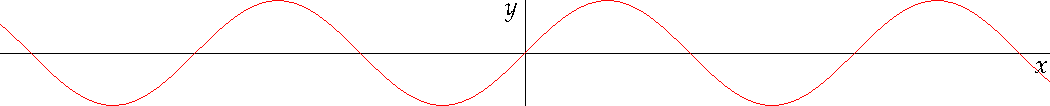
\includegraphics[width=\linewidth]{sine.pdf}%
	\caption{This graph shows $y = \sin x$ from about $x = [-10, 10]$.
	\emph{Notice that this figure takes up the full page width.}}%
	\label{fig:fullfig}%
\end{figure*}

\begin{figure}[h]
	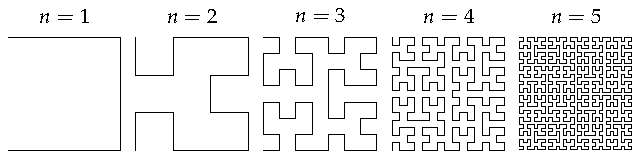
\includegraphics{hilbertcurves.pdf}
	\caption{Hilbert curves of various degrees $n$.
		\emph{Notice that this figure only takes up the main textblock width.}}
	\label{fig:textfig}
	\setfloatalignment{a} % Position the figure caption in the middle of the figure
\end{figure}

The style contains two new environments called \textsf{marginfigure} and \textsf{margintable} which allow you to place a figure or table entirely in the margin. Like side and margin notes, the \textsf{marginfigure} and \textsf{margintable} environments accept an optional \texttt{<offset>} argument that adjusts the vertical position of the figure or table. Figure~\ref{fig:marginfig} is an example of a margin figure that has been moved up due to a clash with Figure~\ref{fig:textfig} above it.

\begin{marginfigure}[-0.75cm]
	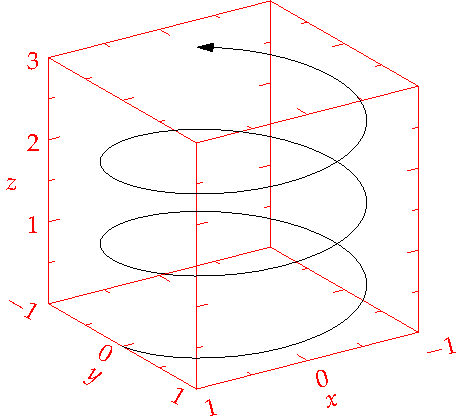
\includegraphics[width=\linewidth]{helix.pdf}
	\caption{This is a margin figure. The helix is defined by $x = \cos(2\pi z)$, $y = \sin(2\pi z)$, and $z = [0, 2.7]$. The figure was drawn using Asymptote (\url{http://asymptote.sf.net/}).}
	\label{fig:marginfig}
\end{marginfigure}

Table~\ref{tab:normaltab} shows a table created with the \texttt{booktabs} package. Notice the lack of vertical rules---they serve only to clutter the table's data.

\begin{table}[ht]
	\centering
	\fontfamily{ppl}\selectfont
	\begin{tabular}{l l}
		\toprule
		Margin                    & Length                          \\
		\midrule
		Paper width               & \unit[8\nicefrac{1}{2}]{inches} \\
		Paper height              & \unit[11]{inches}               \\
		Textblock width           & \unit[6\nicefrac{1}{2}]{inches} \\
		Textblock/sidenote gutter & \unit[\nicefrac{3}{8}]{inches}  \\
		Sidenote width            & \unit[2]{inches}                \\
		\bottomrule
	\end{tabular}
	\caption{Here are the dimensions of the various margins used in the Tufte-handout class when using letterpaper.}
	\label{tab:normaltab}
	\setfloatalignment{b} % Position the table caption at the bottom of the table
\end{table}

%------------------------------------------------

\section{Typography}\label{sec:typography}

\subsection{Typefaces}\label{sec:typefaces}

If the Palatino, \textsf{Helvetica}, and \texttt{Bera Mono} typefaces are installed, this style will use them automatically. Otherwise, it will fall back on the Computer Modern typefaces.

\subsection{Letterspacing}\label{sec:letterspacing}

This style includes two new commands and some improvements on existing commands for letterspacing.

When setting strings of \allcaps{ALL CAPS} or \smallcaps{small caps}, the letter\-spacing---that is, the spacing between the letters---should be increased slightly\cite[-0.25cm]{Bringhurst2005}. The \texttt{\textbackslash allcaps} command has proper letterspacing for strings of \allcaps{FULL CAPITAL LETTERS}, and the \texttt{\textbackslash smallcaps} command has letterspacing for \smallcaps{small capital letters}. These commands will also automatically convert the case of the text to upper- or lowercase, respectively.

The \texttt{\textbackslash textsc} command has also been redefined to include letterspacing. The case of the \texttt{\textbackslash textsc} argument is left as is, however. This allows one to use both uppercase and lowercase letters: \textsc{The Initial Letters Of The Words In This Sentence Are Capitalised.}

%------------------------------------------------

\section{Support}\label{sec:support}

The website for the Tufte-\LaTeX\ packages is located at \url{https://github.com/Tufte-LaTeX/tufte-latex}. On the website, you'll find links to the \smallcaps{svn} repository, mailing lists, bug tracker, and documentation.

%----------------------------------------------------------------------------------------
%	BIBLIOGRAPHY
%----------------------------------------------------------------------------------------

\bibliography{sample.bib} % Use \nobibliography{<bib file>} if you have references but don't want to print a bibliography

\bibliographystyle{plainnat}

%----------------------------------------------------------------------------------------

\end{document}
